\emph{Pobřežní (litorální) zóna} je prostor na rozhraní moře, oceánu, ale i jiné velké vodní plochy (jezero) a souše. Tato zóna zahrnuje jak mělčiny, tak i přilehlou souš. \textcite{demekObecnaGeomorfologie1987} břežní pásmo definuje jako pás území ležící na styku pevniny a světového oceánu ve kterém se uskutečňuje interakce mezi pevninou a oceánem. \emph{Dolní hranice} je definována jako místo na dně, kde končí geomorfologická schopnost i největších vln při bouřích. \emph{Horní hranice} je vymezena \emph{přímořskou čarou} -- linií maximálního působení vln při příboji. 

\begin{figure*}[h]
	\centering
	\includegraphics[width=0.9\linewidth]{obrazky/marine/pobrezi}
	\caption{Vymezení pobřežních zón (upraveno podle \textcite{birdCoastalGeomorphologyIntroduction2008}).
		}
	\label{fig:pobrezi}
\end{figure*}

Charakter a modelace břežního pásma je ovlivněna aktivními a pasivními činiteli. Do \emph{aktivních činitelů} řadíme ty, které mají dostatečnou kinetickou energii pro modelaci břežního pásma. Jedná se o vlny, vlnové proudy, výčasové proudy, ale i biotu. Mezi \emph{pasivní činitele} řadíme morfostrukturu, reliéf, klima apod. 

\section{Vlnění}
Vlny jsou hlavním aktivním činitelem, který utváří pobřeží. Jsou popisovány několika parametry. Vlnová délka ($\lambda$ nebo L) je vzdálenost mezi dvěma hřbety vln. Perioda vlny ($T$) je čas, který uplyne než se následující vlna dostane do pozice vlny předchozí. Rychlost vlny ($V$) je daná rovnicí $V = \lambda/T$.  Výška vlny nebo také amplituda ($H$) je vertikální vzdálenost mezi nejnižším místem (dolem) a hřbetem vlny. Vlnění směrem do hloubky postupně ustává a zaniká v hloubce rovnající se polovině vlnové délky. Tuto hloubku označujeme jako \emph{báze vlny}. Vrchol  vlny se nazývá hřbet a nejnižší bod se označuje jako důl nebo vpadlina. 

\begin{figure*}[h]
	\centering
	\includegraphics[width=0.8\linewidth]{obrazky/marine/vlny}
	\caption{Popis vlny a jejích charakteristik}
	\label{fig:vlny}
\end{figure*}



\subsection{Eolické vlny}
Vlny vznikají rozpohybováním vodní masy proudícím vzduchem. Část energie větru vanoucího nad vodní hladinou je přenášena na vodní těleso. 

Vznik vln ovlivňují tři základní faktory:
\begin{enumerate}
	\item délka trvání větru o určitém směru
	\item rychlost větru
	\item náběhová vzdálenost větru
\end{enumerate}

Silný vítr o dlouhém trvání, který vane na dlouhou vzdálenost vytváří velké vlny s vysokou kinetickou energií. 

V hlubokých vodách, tedy tam, kde báze vlny neprotíná dno probíhá pohyb molekul po kružnici. Směrem do hloubky se jejich průměr zmenšuje. Toto vlnění označujeme jako \emph{vlnění hluboké vody}. Když vlna dosáhne mělčích vod (hloubka $< 0,5\lambda$), začíná vlna interagovat se dnem. Pohyb částic již neprobíhá po kružnicích, ale po elipsách. Část energie vln je vynaložena na transport sypkého materiálu na dně a modelaci dna. Dochází ke zkracování vln a jejich zpomalování. Výška vlny ale naopak narůstá a čelní svah vlny se stává strmějším. Zvyšuje se tak poměr mezi výškou vlny a vlnovou délkou ($H/\lambda$). Směrem k pobřeží se tato transformace zesiluje. Když $H/\lambda$ překročí $1/7$, hřbet vlny ztrácí oporu a dochází k lámání vlny. Vzniká tak \emph{příboj} (\textit{surf}), který mění potenciální energii vlny na kinetickou. Způsob jakým se vlna láme je dán strmostí vlny a sklonem pobřeží.

\begin{figure*}[h]
	\centering
	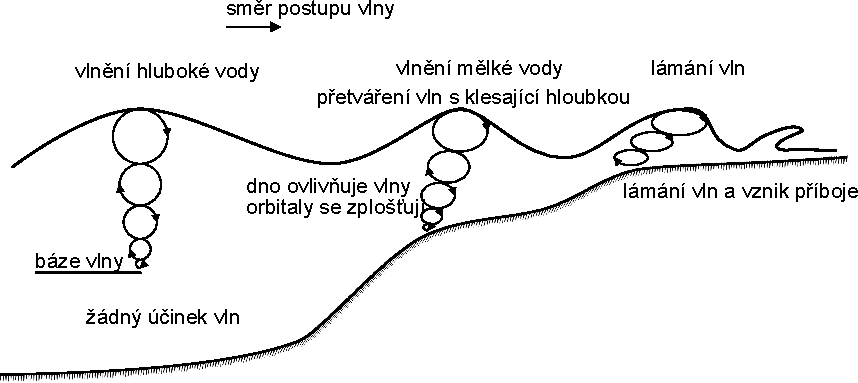
\includegraphics[width=0.8\linewidth]{obrazky/marine/vlny_transformace}
	\caption{Vlny hluboké vlny a jejich transformace postupem ke břehu}
	\label{fig:vlnytransformace}
\end{figure*}

Vlny mají tendenci ohýbat své čelo paralelně s pobřežím -- dochází k tzv. \emph{refrakci vln}. U zálivů se vlny rozšiřují, čímž se jejich energie snižuje. U mysů se naopak vlny stlačují k sobě, čímž se energie koncentruje.
\subsection{Bouřkové vlny}
Dalším typem je \emph{bouřkové vlnění} (\textit{storm surges)}, které vzniká kombinací extrémně nízkého tlaku, silného větru a přílivu. 
 
\subsection{Seismické mořské vlny}
V důsledku zemětřesení mohou vzniknout vlny \emph{tsunami}. Jejich vznik je spojen s vertikálním pohybem oceánského dna. Toto vlnění je charakteristické malou amplitudou, extrémní délkou a rychlostí. Na širém oceánu je tato vlna neznatelná. Dorazí-li však k pobřeží, dojde k razantnímu zkrácení vlny a nárůstu její výšky. 

\section{Příboj}
Směrem k pobřeží se postupující vlny stávají příkřejšími až převislými - dochází k lomu vlny a vzniku příboje resp. příbojového proudu (příboj). Charakter příboje je ovlivněn sklonem pobřeží. Mírné písčité pláže jsou typické příbojem typu \textit{spilling breaker}. Vlna se postupně bortí do podoby zpěněné nerovnoměrné vlnové fronty. Voda pak v poklidu odtéká z pláže. Zcela kontrastní jsou tzv. \textit{plunging breakers} a \textit{surging breakers}. Vznikají na březích se strmějším dnem. Rysem \textit{plunging breaker} je lámání vrcholu vlny. Vlna se překlápí dopředu a padá na hladinu. Vzniká trubulentní vodní masa vody. \textit{Surging breaker} je třetí typ. Tímto divokým příbojem jsou charakteristické strmé pláže. Nedochází k lomu vrcholu vlny, ale ta naráží plnou silou na pláž.

\section{Vlnové proudy}
Postupující vlny k pobřeží jsou transformovány do dvou složek -- \emph{příčné} a \emph{podélné}. Příčnou složku tvoří vlnové proudy směrem k pobřeží a zpětné kompenzační (náporové) proudy (\textit{rip current}). Zpětné náporové proudy jsou poměrně úzké, ale velice rychlé (až několik \si{\metre\per\second}), proto jsou schopné unášet velké množství materiálu z břežního pásma \parencite{demekObecnaGeomorfologie1987}. 

Podélná složka je tvořena \emph{příbřežními} proudy. Ty nejlépe fungují při postupu vln šikmo k pobřeží. Tyto proudy jsou důležité pro přemísťování materiálu podél pobřeží.

\section{Výčasové proudy}
Výčasové proudy se skládají z přílivových a odlivových proudů. Přílivové proudy jsou velice účinné v průlivech a estuáriích. Na otevřeném oceáně mají výčasové proudy rychlosti okolo \SI{0,3}{\metre\per\second}. V průlivech jejich rychlost narůstá až k \SI{7}{\metre\per\second}.

\section{Pobřežní procesy}
\subsubsection{Pobřežní zvětrávání a eroze}
Zvětrávání na pobřeží je umocněno opakovaným zvhlčováním a schnutím hornin. Velký vliv má i solné zvětrávání a chemické zvětrávání (hlavně v tropech). Typ hornin má samozřejmě významný vliv na intenzitu zvětrávacích procesů. Např. solné zvětrávání bude probíhat intenzivněji v horninách nasákavých, které mohou absorbovat mořskou vodu. Rozpouštění vápenců na pobřeží je intenzivní v tropických oblastech.

Pobřežní erozi nazýváme souhrnně \emph{abraze}. Hlavním erozním činitelem na pobřeží jsou vlny. Jejich účinek je ovlivněn charakterem pobřeží a horninami. V případě strmých útesů nedochází k lámání vln a ty se bez většího geomorfologického účinku odráží zpět. Mnohem silnější erozní účinek mají vlny, které se lámou. Dochází tam ke kombinaci účinku samotné dopadající vlny a vzduchu, který je stlačen mezi vlnou a břehem. Výsledkem je vytrhávání a vyrývání kusů hornin. Nejnáchylnější na erozi jsou slabě zpevněné sedimenty a značně rozpukané skalní horniny.

Nezanedbatelný podíl na pobřežní erozi mají živé organizmy (různí měkkýši, mořské houby), které se zavrtávají do hornin a tak je rozrušují. 

\subsubsection{Pohyb a depozice sedimentů}
Hlavní zdrojnice sedimentů na pobřeží jsou samotné pobřežní formy reliéfu, oblasti dál na pevnině a dál v moři. Významným zdrojem materiálu zejména v místech se silným příbojem mohou být útesy, které pokud jsou tvořeny měkkými horninami snadno erodují. Dalším zdrojem mohou být svahové procesy. Útesy podkopávané příbojem kolabují, čímž se do pobřežního systému dostává velké množství materiálu. V polárních oblastech se intenzivně uplatňuje termoeroze. Největším zdrojem materiálu jsou ale vodní toky.  Materiál na pobřeží se ale může dostávat i v důsledku silných bouří nebo vln tsunami.

Hlavní směr pohybu sedimentů je podél pobřeží v důsledku příbřežních proudů. Rychlost je závislá zejména na orientaci vln přicházejících k pobřeží.

\section{Pobřežní formy reliéfu}

\subsection{Erozní pobřeží}
Skalnatá pobřeží mohou nabývat dvou základních forem. První představuje skalnatý útes -- \emph{abrazní srub}, který se noří hluboko pod mořskou hladinu. Tento typ pobřeží nemá žádnou pláž a energie příboje se vybíjí přímo na útesech. Pobřeží je tvořené odolnými (zejména krystalickými) horninami. Strmé útesy mohly vzniknout tektonickými procesy případně vodní nebo ledovcovou erozí a následným zaplavením (např. pobřeží Norska). Druhá forma je charakteristická abrazním srubem, který přechází do \emph{abrazní terasy} (Obr. \ref{fig:abrazni}). Abrazní terasa (Obr. \ref{fig:abrazni_terasa}) je horizontální nebo mírně ukloněná plošina. Vzniká postupným ústupem abrazního srubu. Na abrazní plošině je velmi malé množství materiálu, který je neustále v pohybu.

\begin{figure}[h]
	\centering
	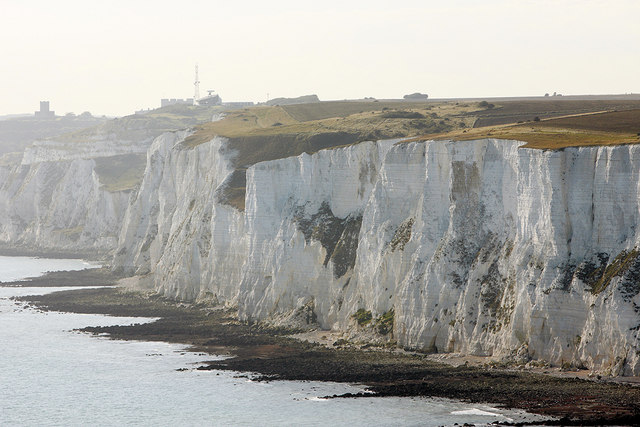
\includegraphics[width=1\linewidth]{obrazky/marine/abrazni}
	\caption{Ukázka abrazního pobřeží. Abrazní srub a abrazní terasa. Letecký snímek Doverských útesů (Autor: Alan Duncan, CC BY-SA 2.0)}
	\label{fig:abrazni}
\end{figure}

\emph{Útes} (\textit{cliff}) je strmý až převislý svah na pobřeží. Při úpatí útesu je \emph{abrazní výklenek}, který je vytvořen abrazní činností vln. Útes může mít několik abrazních výklenků, které jsou dokladem hladiny moře v minulosti. Postupnou erozí útesů v důsledku abraze, ale i gravitačních procesů, dochází k ústupu útesů. Podoba útesu je dána charakterem hornin, jejich strukturou a odolností vůči abrazi a zvětrávání. 

Nerovnoměrným ústupem abrazního srubu můžou vznikat \emph{abrazní brány}, \emph{abrazní jeskyně}, ale i zcela izolované \emph{abrazní jehly} či \emph{pilíře} (Obr. \ref{fig:apostol}).

\begin{figure}[h]
	\centering
	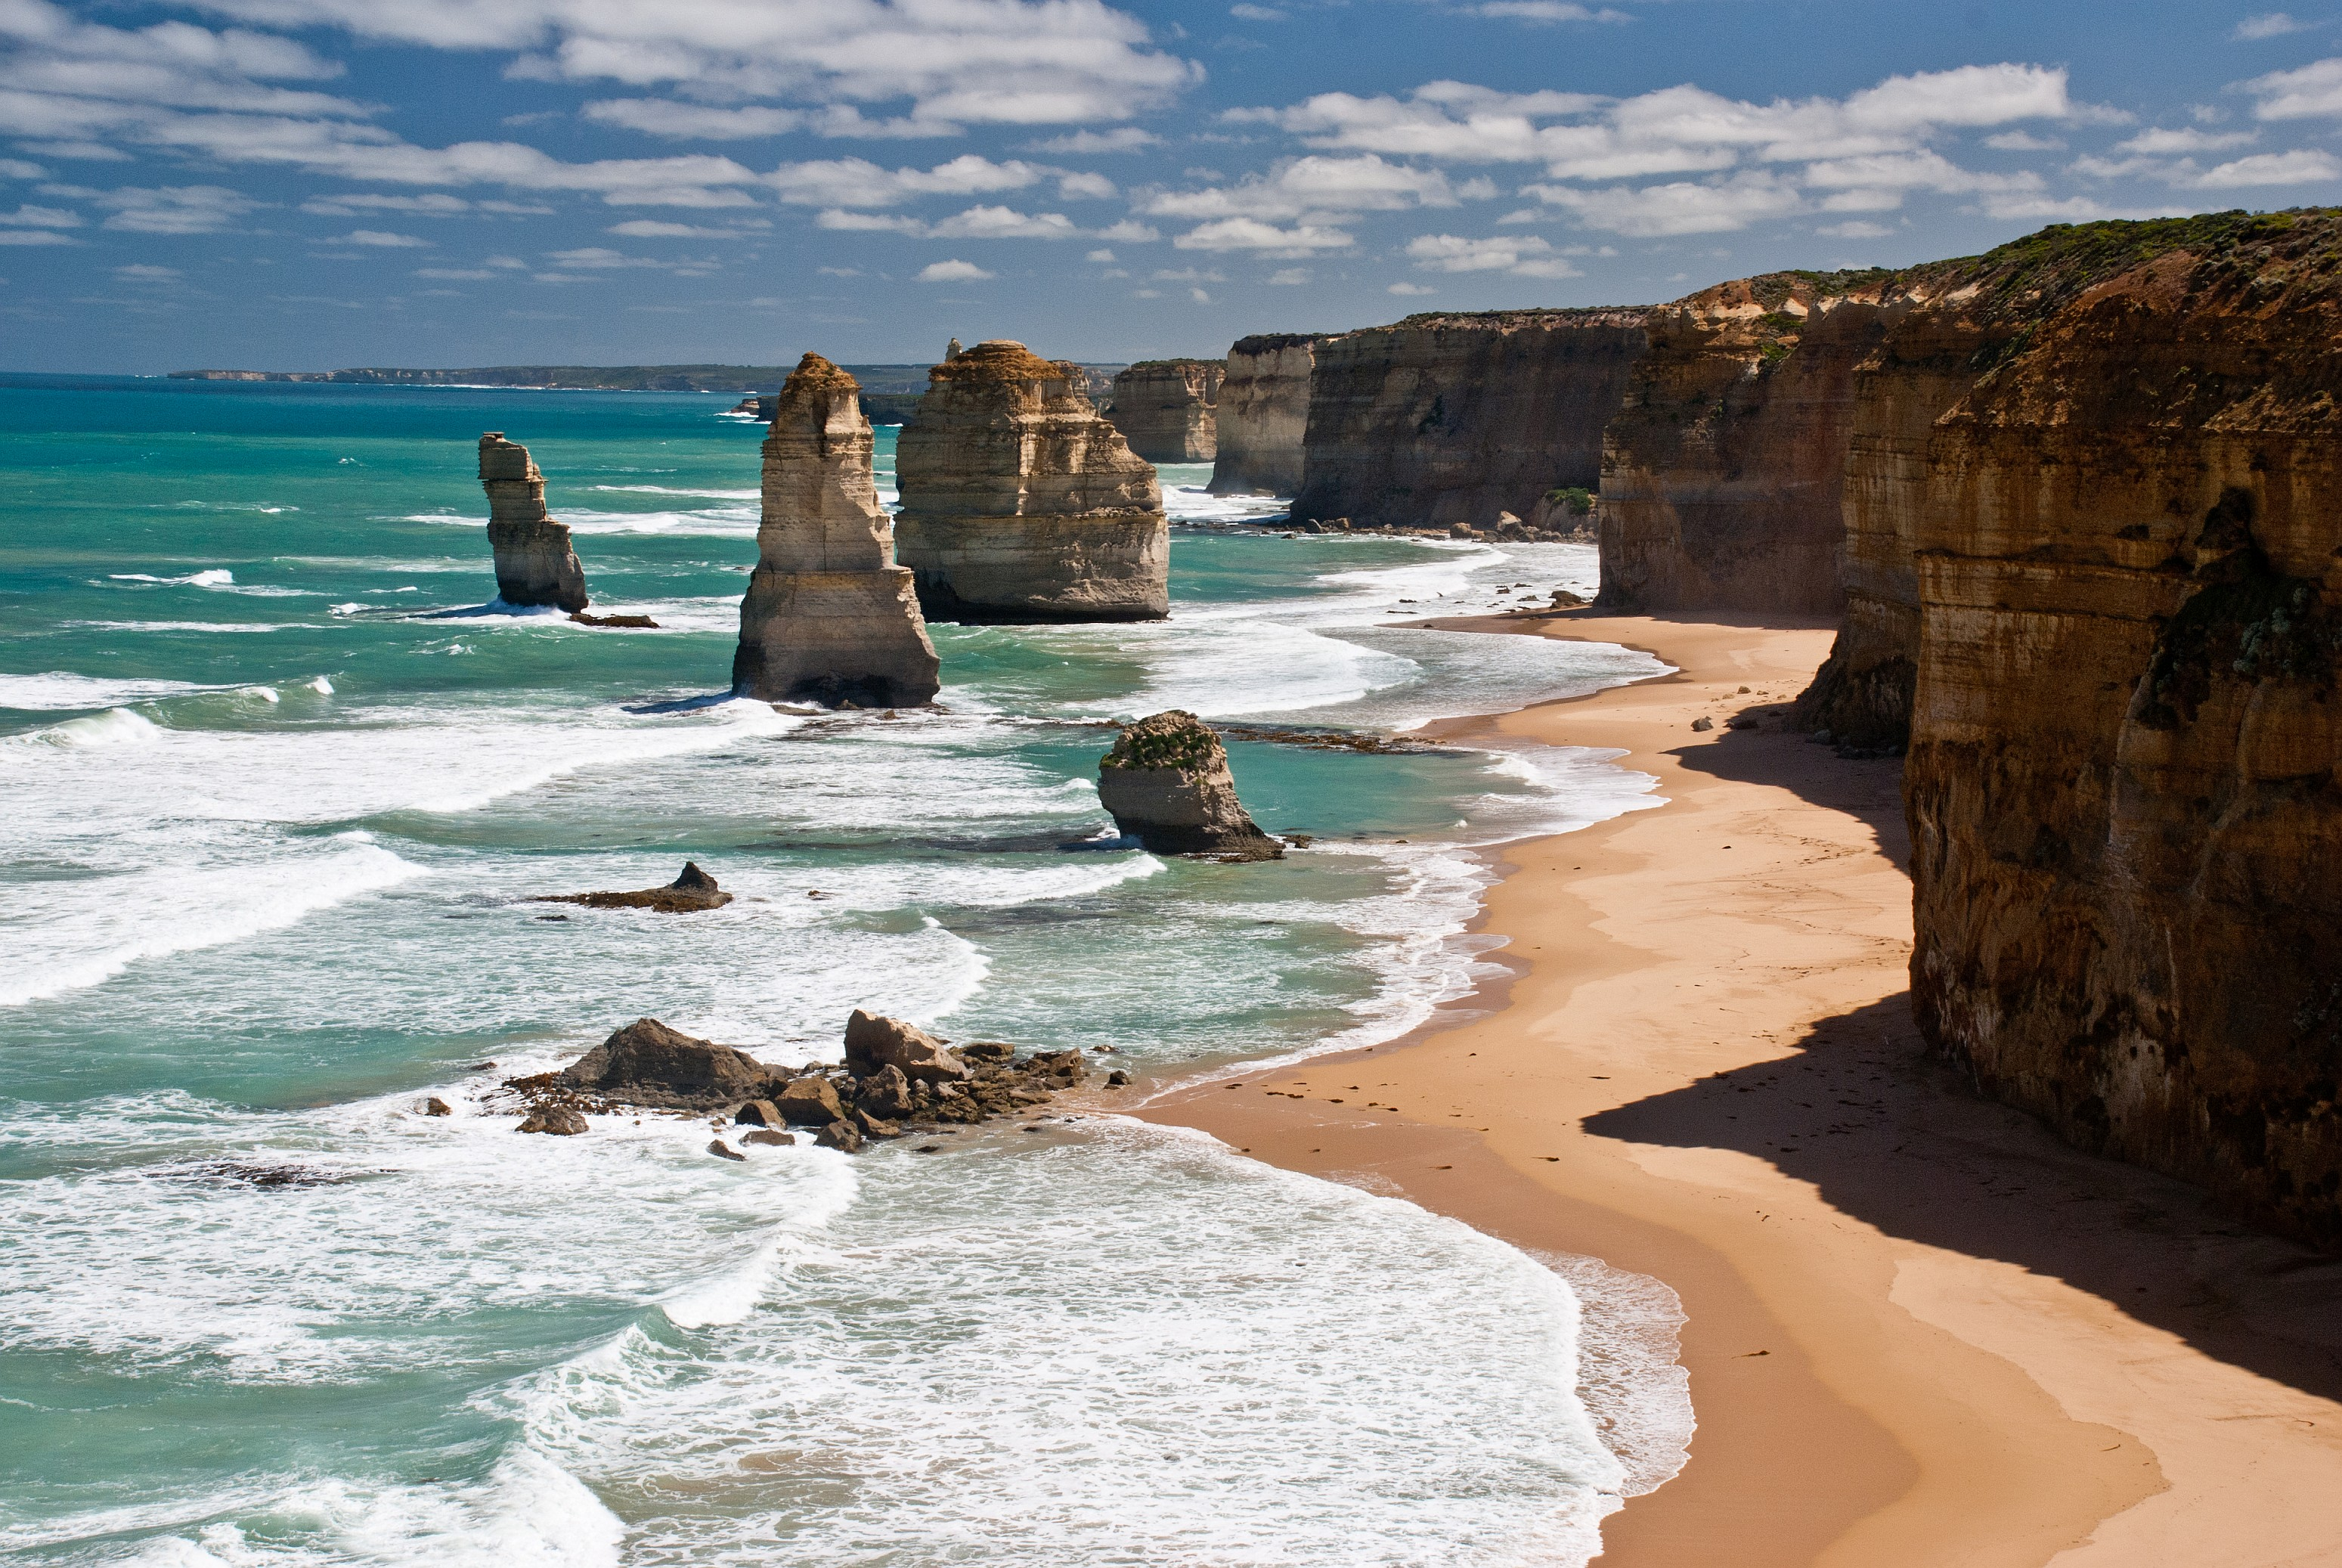
\includegraphics[width=1\linewidth]{obrazky/marine/apostolove}
	\caption{Abrazní pilíře, Dvanáct apoštolů, Austrálie. V popředí je pozůstatek jednoho z pilířů, který se zřítil v roce 2005 (Autor: Richard Mikalsen, CC BY-SA 3.0, via Wikimedia Commons)}
	\label{fig:apostol}
\end{figure}

\begin{figure}[h]
	\centering
	\includegraphics[width=1\linewidth]{obrazky/marine/utesy_terasy}
	\caption{Možné podoby abrazních teras (upraveno podle \textcite{birdCoastalGeomorphologyIntroduction2008})}
	\label{fig:abrazni_terasa}
\end{figure}



\subsection{Akumulační tvary}
\subsubsection{Pláže}
Pláž (\textit{beach}) je typickým akumulačním tvarem pobřeží. Pláže mohou být písečné, štěrkové i oblázkové. Významnou složkou materiálu tvořícího pláže je i organický materiál, a to zejména karbonáty (např. schránky živočichů). Velikost klastů má významný vliv na podobu pláže. Příbojový proud unáší materiál k pobřeží a jak postupně ztrácí energii, tak dochází k postupné sedimentaci a tedy i třídění sedimentů. Směrem k souši se materiál zjemňuje. 

Na pláži můžeme vymezit další formy jako je například \emph{bouřkový stupeň}, \emph{plážová terasa} či \emph{předbřežní val}

\subsubsection{Písečné kosy a tomboly}
V tzv. vlnovém stínu vznikají různé \emph{písečné výběžky} (široké) a úzké \emph{kosy} (\textit{spit}). Nejčastěji vznikají při ústí řek a v místech změny směru pobřeží. Asi nejznámější kosou je Hel v Polsku.
\emph{Tombola} je písečná akumulace, která spojuje dva kusy pevniny.

\begin{figure}[h]
	\centering
	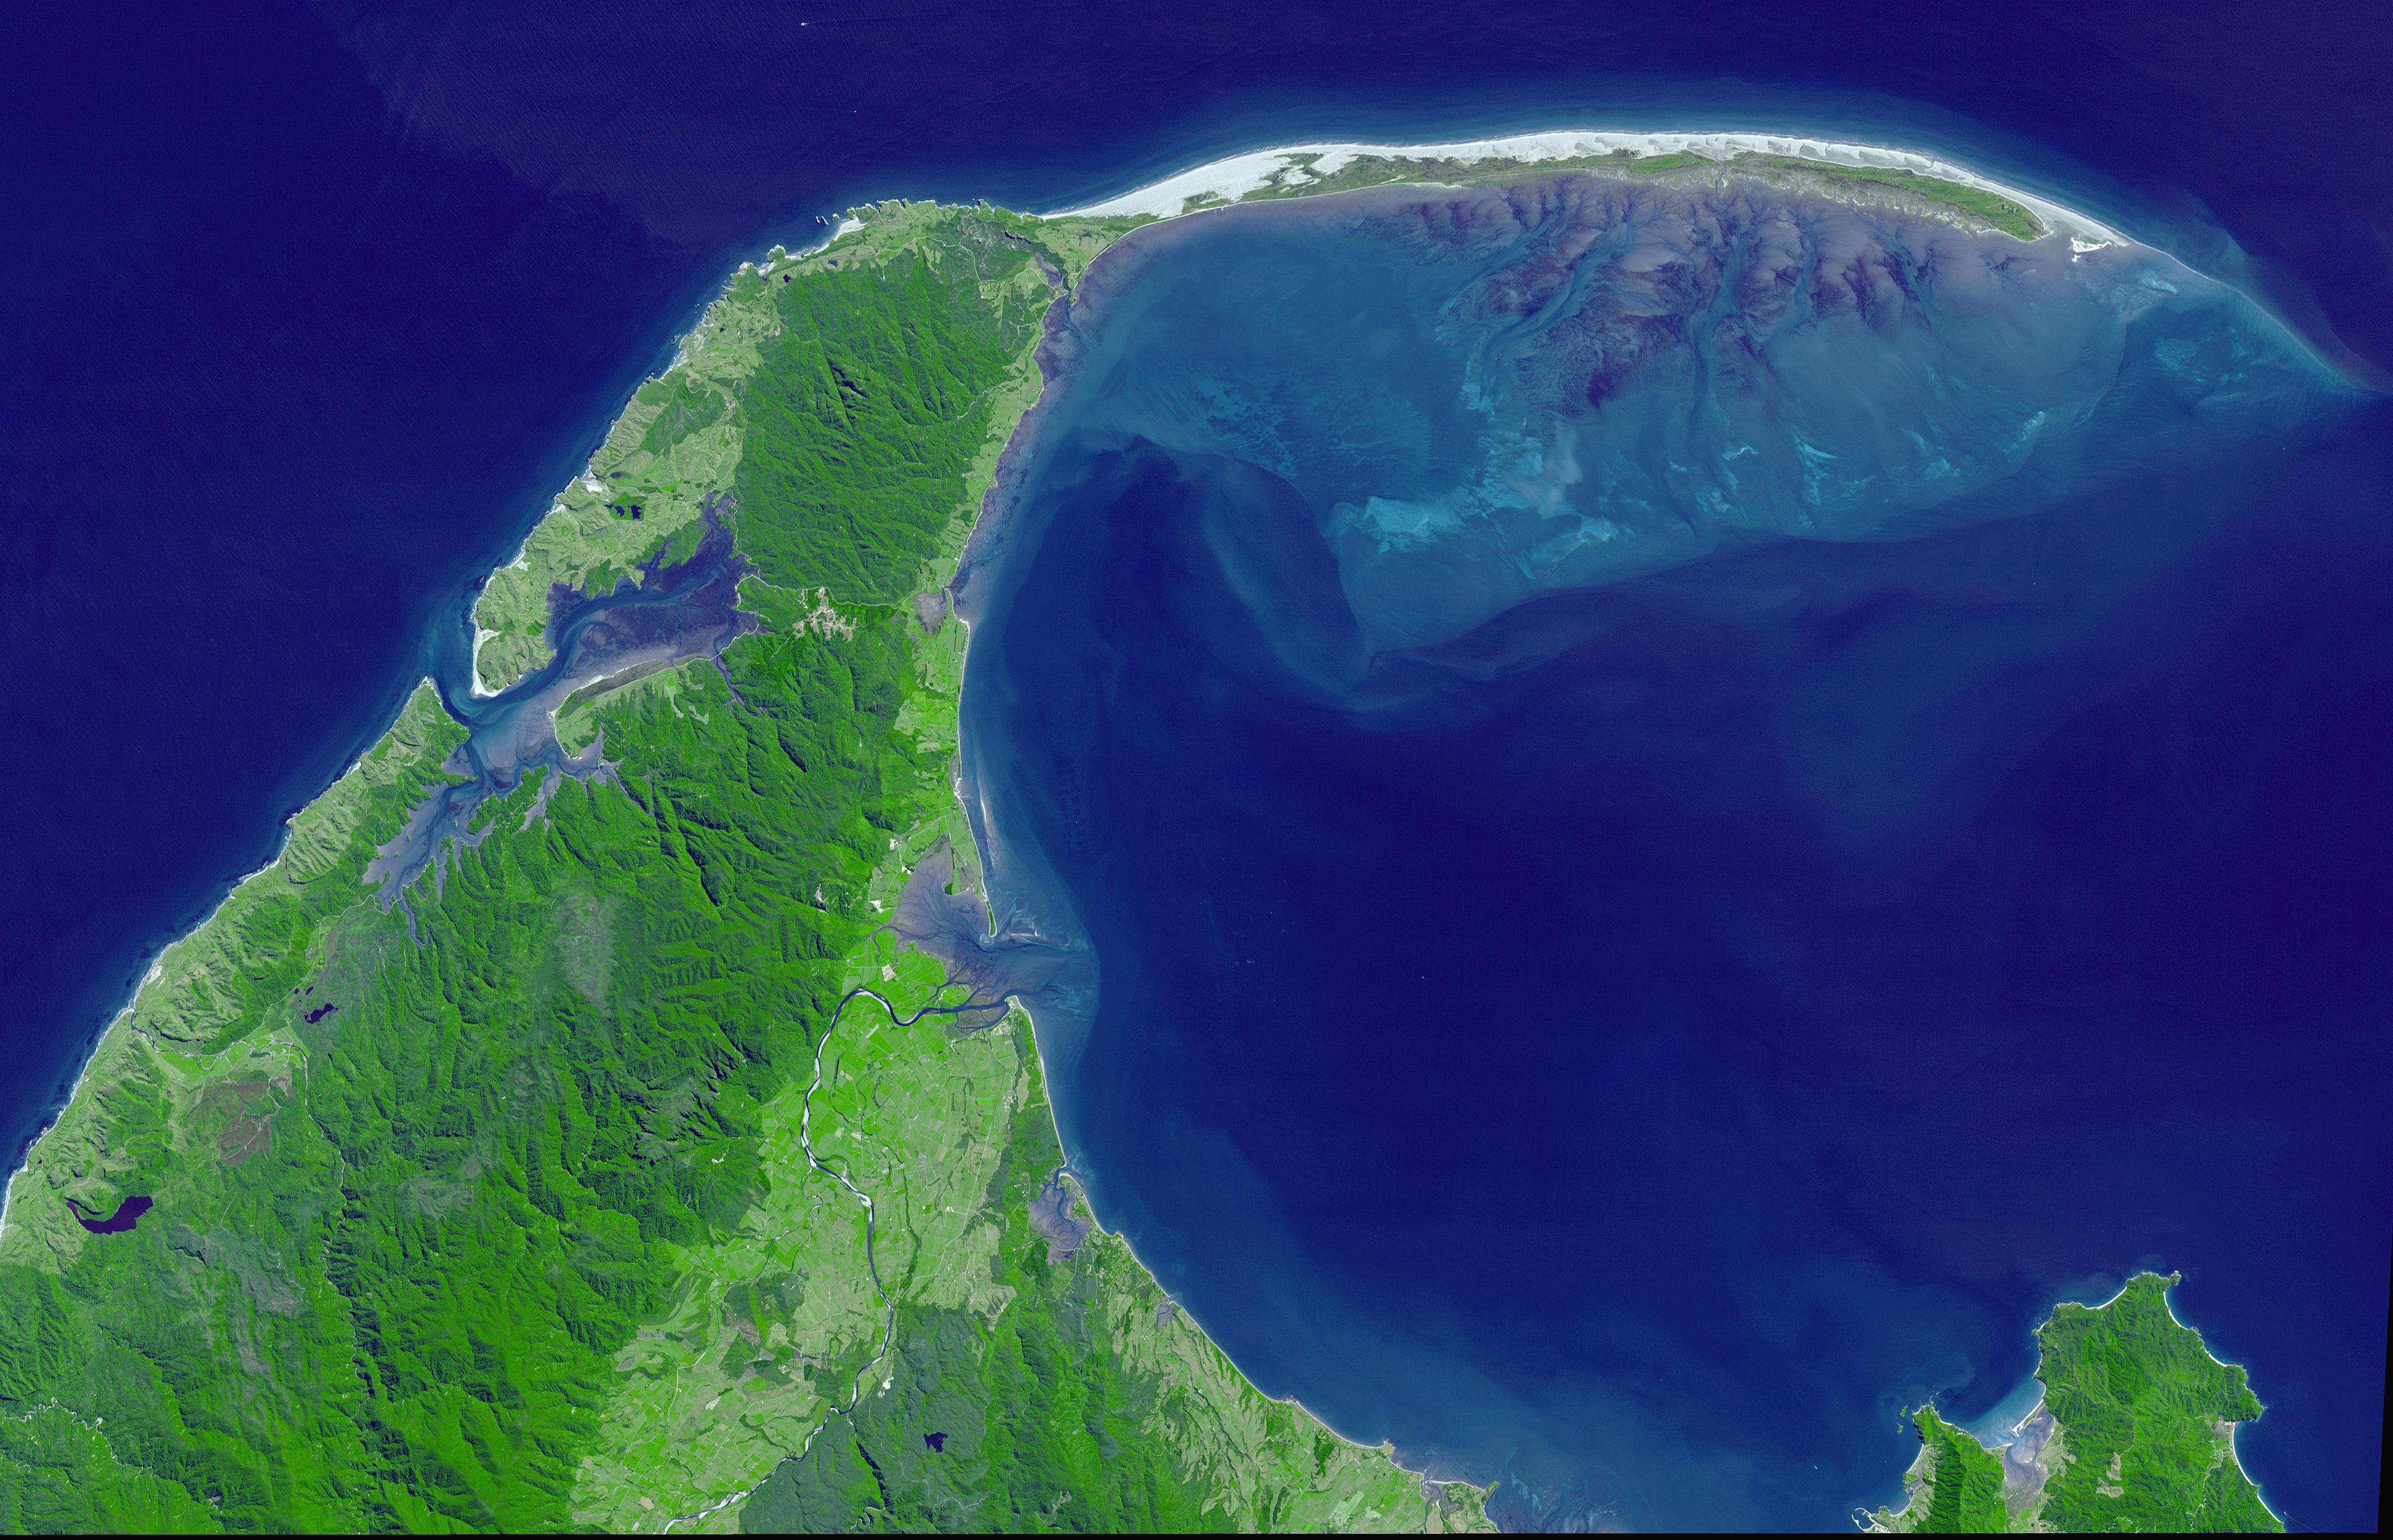
\includegraphics[width=1\linewidth]{obrazky/marine/kosa}]
	\caption{Farewell Spit -- kosa na severním výběžku Jižního ostrova Nového Zélandu (Zdroj: NASA, volné dílo)}
	\label{fig:kosa}
\end{figure}

\subsubsection{Bariérové ostrovy}
\emph{Bariérové ostrovy} jsou nízké ostrovy protáhlé ve směru pevniny, od které jsou odděleny \emph{lagunou}. Bariérové ostrovy mohou nabývat rozličných rozměrů. Malé ostrovy mají šířku několik metrů a délku v rámci stovek metrů. Největší nabývají šířky přes kilometr. Na největších ostrovech vzniká i systém písečných dun. Výskyt bariérových ostrovů je vázán na oblasti s velice mírným pobřežím a malým rozpětím přílivu a odlivu.

\subsubsection{Přílivové plošiny a marše}
Rozsáhlé ploché akumulační formy, které jsou zaplavované během přílivu se označují jako \emph{přílivové plošiny} nebo {watty}. Jsou tvořeny siltem a jílem. Velký podíl má i organická hmota. Postupnou agradací přílivových plošin se snižuje dosah průměrných přílivů, což umožňuje rozvoj vegetace, další agradaci a vznik půdy. Watyy tak přechází v \emph{marše}, které jsou zaplavovány jen při skočném přílivu. Pokud i ty přestanou být pod vlivem přílivu, vzniká pobřežní nížina. 

\begin{figure}[h]
	\centering
	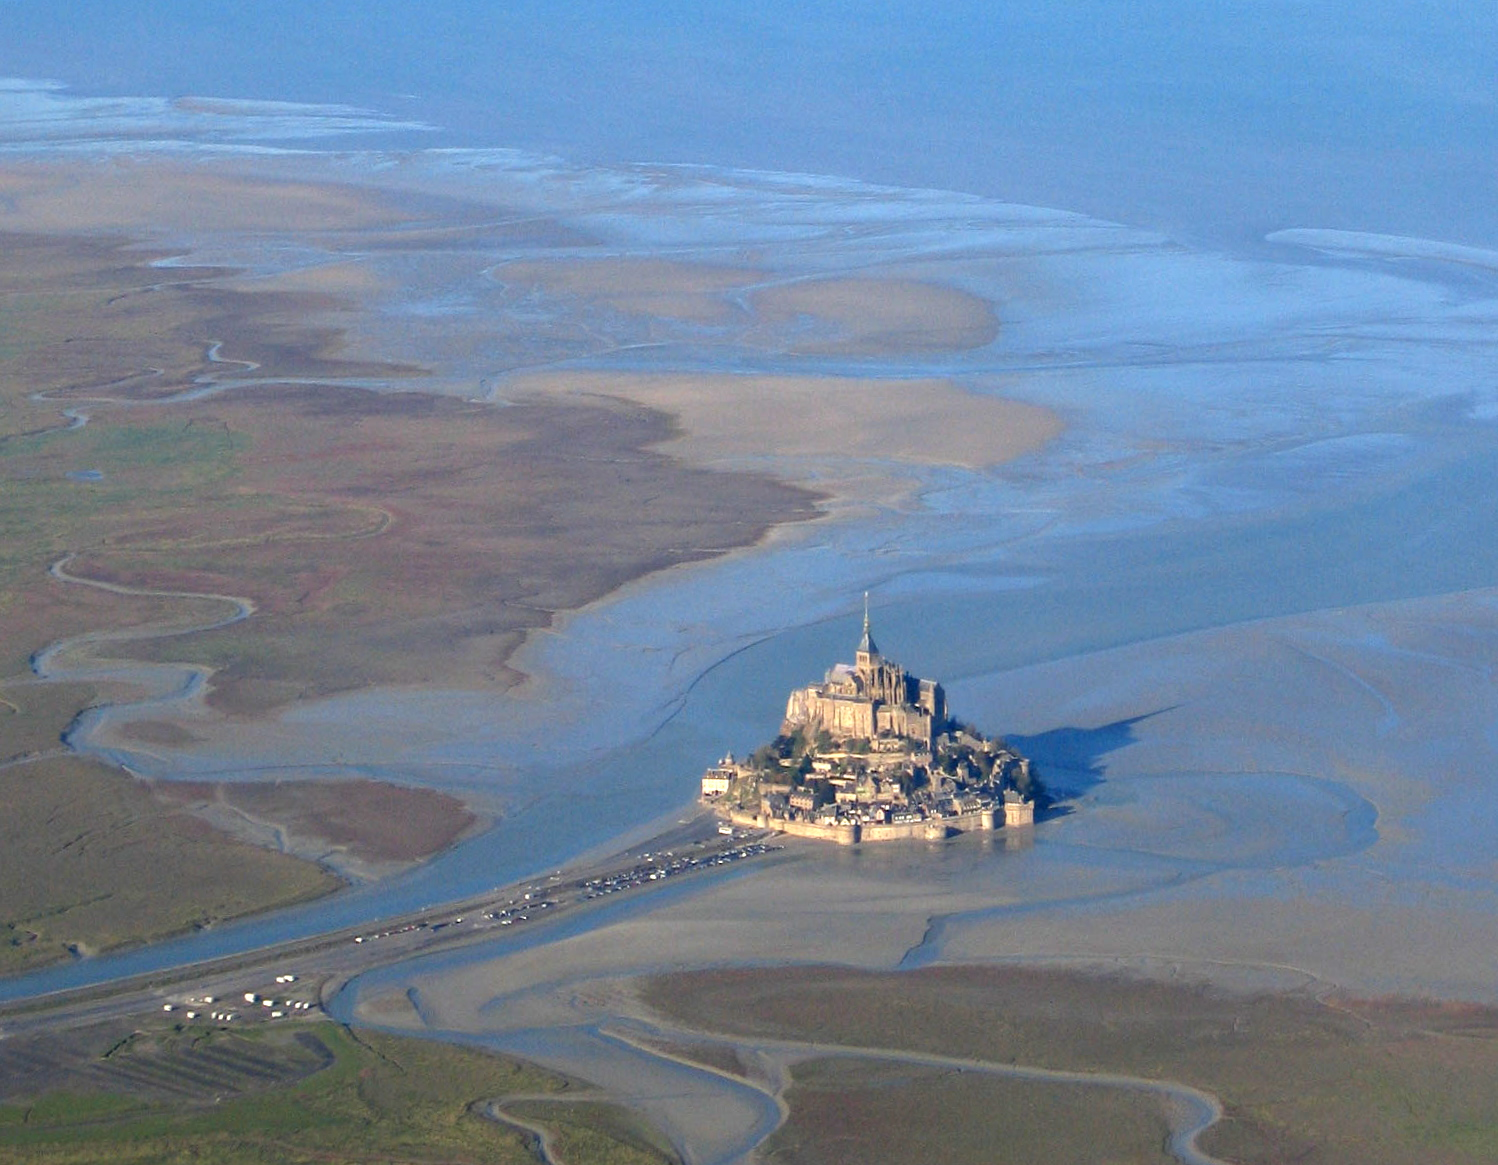
\includegraphics[width=1\linewidth]{obrazky/marine/watty}
	\caption{Pohled na příbřežní plošinu s ostrovem Mount Saint-Michel. (volné dílo, via Wikimedia Commons)}
	\label{fig:watty}
\end{figure}

\subsubsection{Říční delta}
\emph{Delta} je akumulační tvar vznikající při ústí řek do jezer, moří či oceánů. Vodní tok při zaústění do vodního tělesa se rozšiřuje a razantně klesá rychlost proudění. To způsobuje snížení transportní kapacity a dochází k splavenin. Důležitou podmínkou pro vznik delty je, aby řeka přinášela velké množství materiálu, které pobřežní procesy nejsou schopné odnést. 

Sedimentace dnových splavenin nastává okamžitě. Sedimentace plavenin (materiálu v suspenzi) je ovlivněna poměrem hustoty vodního toku a mořské či jezerní vody. V případě stejné hustoty obou vod dochází k rychlému promíchání a k okamžité sedimentaci. Toto se nastává zejména u sladkých vod, tedy když řeka vtéká do jezera. Druhý případ je, pokud má voda v řece větší hustotu než je voda v tělese, do kterého vtéká. Hustší říční voda se noří pod vodu s nižší hustotou a v podobě proudu u dna transportuje sedimenty daleko od břehu. K vývoji delty tak nemůže docházet. Toto nastává když například velice studená řeka vtéká (voda má nejvyšší hustotu při \SI{4}{\celsius}) do teplého jezera. Poslední možnou variantu je, když říční voda má menší hustotu než voda, do které vtéká. V tomto případě se říční voda rozlije po povrchu a pokud transportuje velké množství splavenin, tak vytváří snadno identifikovatelné mračno, které postupuje daleko od břehu, než se voda dostatečně promíchá. Tato varianta je typické pro případy, kdy řeka (sladká voda, nízká hustota) vtéká do moře (slaná voda, vysoká hustota).

Nejjednodušší podoba delty je tzv. \emph{Gilbertova delta} (pojmenovaná podle amerického geologa Grove Karl Gilberta). Tyto delty vznikají zejména v jezerech, kde nedochází ke komplexním vlivům dalších procesů (příboje, slapových jevů, mořských proudů). Jedná se tedy o deltu s dominantní fluviální sedimentací. V sedimentech delty můžeme rozlišit tři základní jednotky: topset, foreset, bottomset. \emph{Topset} jsou horní, (sub)horizontálně uložené sedimenty. \emph{Foreset} jsou šikmé, do jezera se uklánějící vrstvy. Postupným budováním foresetu dochází k rozšiřování delty. \emph{Topset} jsou (sub)horizontální vrstvy uložené v hluboké vodě na okraji delty. Jsou tvořené zejména jemnozrnným materiálem.

\begin{figure}[h]
	\centering
	\includegraphics[width=1\linewidth]{obrazky/fluvial/gilbert_delta}
	\caption{Schéma jednoduché (Gilbertovy) delty}
	\label{fig:gilbertdelta}
\end{figure}

Delty vznikající u ústí řek do moří a oceánů jsou mnohem komplexnější jak svým vzhledem, tak sedimentací. Jejich podoba je závislá na množství sedimentů, které řeka unáší, síle proudu řeky a mořských proudů, energii vln a slapových jevů. Můžeme rozlišit tři základní typy \parencite{boggsPrinciplesSedimentologyStratigraphy2014}. \emph{Delty s dominancí říční sedimentace} se nacházejí v oblastech, kde vlny mají nízkou energii a rozdíl hladin během přílivu a odlivu je malý. Tyto delty mají charakteristický tvar \enquote{text}{ptačí nohy}. Příkladem je delta řeky Mississippi. \emph{Delta s dominancí vlnění} je typ delty, kde distribuce sedimentů je řízena vlněním. Většina sedimentů, které se dostávají řekou do moře je proudy distribuovaná podél pobřeží. Delta Nilu se řadí do této skupiny. \emph{Delty s dominancí slapových jevů} vznikají v oblastech s výrazným dmutím a slabým vlivem vln. Delta je formována silnými slapovými proudy, které působí erozně. Delta má podobu ostrovů, které jsou od sebe rozdělené širokými kanály.

\begin{figure*}[h]
	\centering
	\includegraphics[width=1\linewidth]{obrazky/fluvial/delty}
	\caption{Typy delt v závislosti na převládajících procesech (Upraveno podle \textcite{seyboldModelingRiverDelta2007})}
	\label{fig:delty}
\end{figure*}

\subsubsection{Estuáry}
Estuáry jsou nálevkovitá ústí řek do moří. Mohou vznikat v důsledku transgrese -- zvednutí hladiny světového oceánu a zaplavením ústí řeky dál do vnitrozemí. Dalším typem jsou fjordy, což jsou zaplavená ledovcová údolí (trogy). Estuáry mohou mít i tektonický původ. 

\begin{figure}[h]
	\centering
	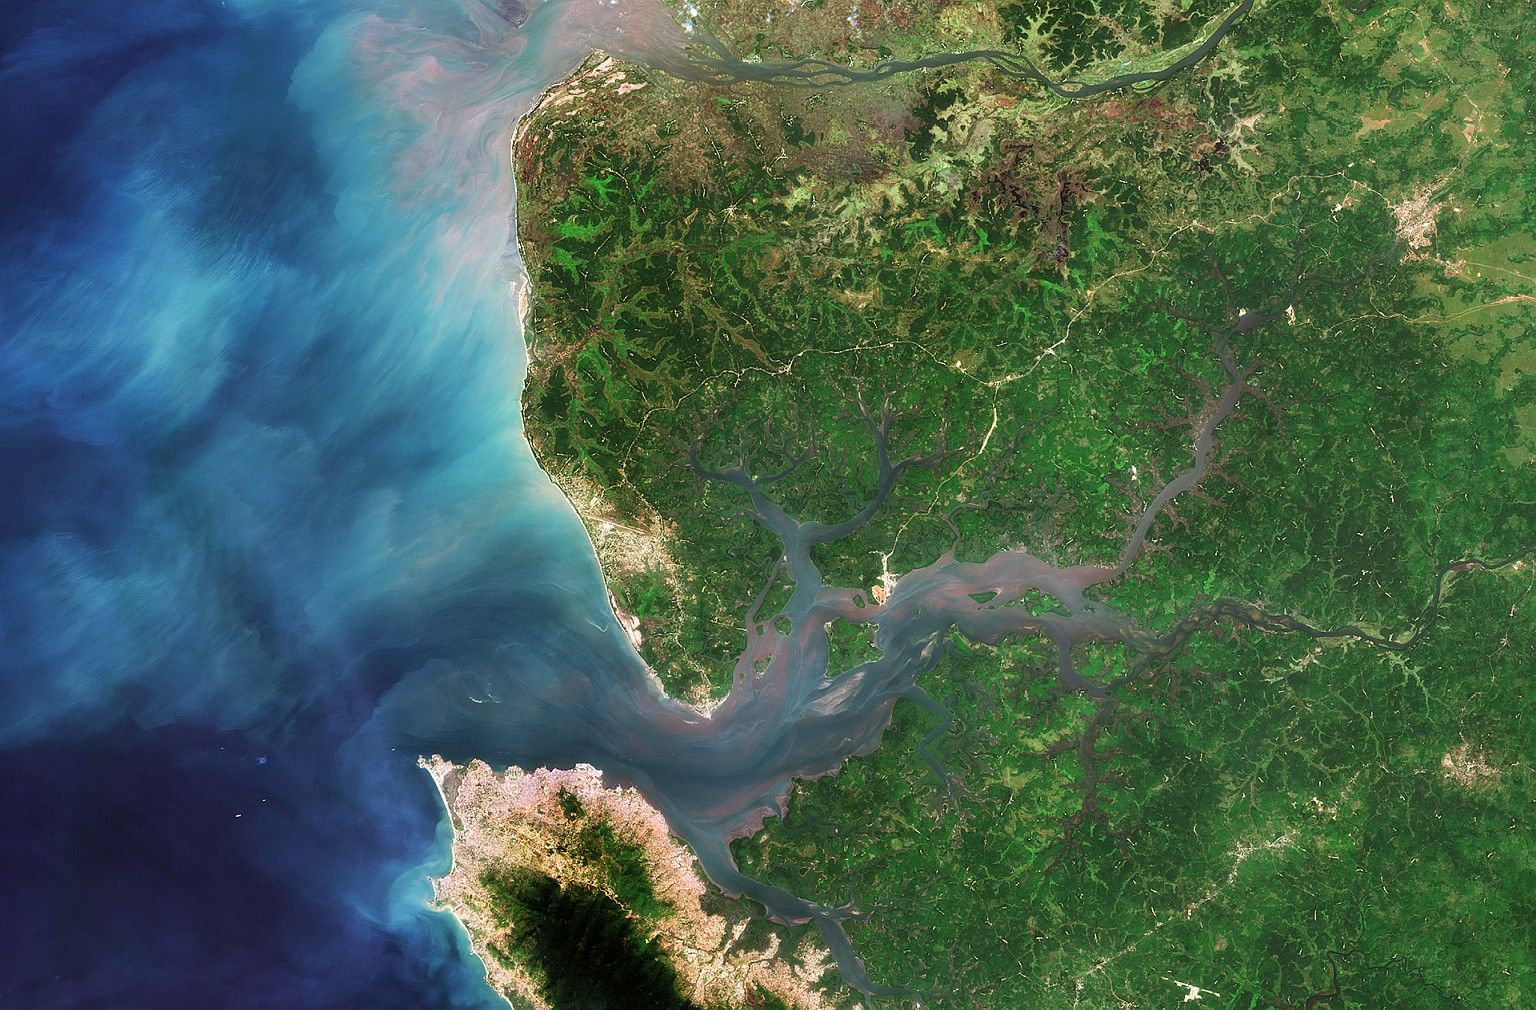
\includegraphics[width=1\linewidth]{obrazky/marine/estuary}
	\caption{Estuár řeky Sierra Leone v Západní Africe. (Zdroj: Copernicus Sentinel data (2015)/ESA,CC BY-SA 3.0 IGO )}
	\label{fig:estuary}
\end{figure}

%\subsection{Marše a mangrovové porosty}
%
%
%\subsection{Biogenní procesy a tvary}

\subsubsection{Korálové útesy}
\emph{Korálové útesy} jsou podmořské skalnaté hřbety v mělkých vodách a vzniklé činností organismů -- zejména korálů, ale i vápnitých řas. Vznik korálových útesů je limitován environmentálními nároky korálů. Optimální teplota moře se pohybuje v intervalu \SIrange{25}{29}{\celsius}. Světelné podmínky v moři omezují růst korálů na maximální hloubku okolo \SI{90}{\metre}, nejintenzivnější růst probíhá do hloubky \SI{20}{\metre}. 

Korálové ptesy rozlišujeme na lemové, bariérové a atolové. \emph{Lemové útesy} se nacházejí v blízkosti břežní čáry. \emph{Bariérové útesy} vytváří valy, které jsou od pobřeží oddělené lagunou. Příkladem je Velký bariérový útes v Austrálii. \emph{Atoly} (obr. \ref{fig:atol}) jsou korálové útesy, které zcela nebo z větší části obkružují lagunu.

\begin{figure}[h]
	\centering
	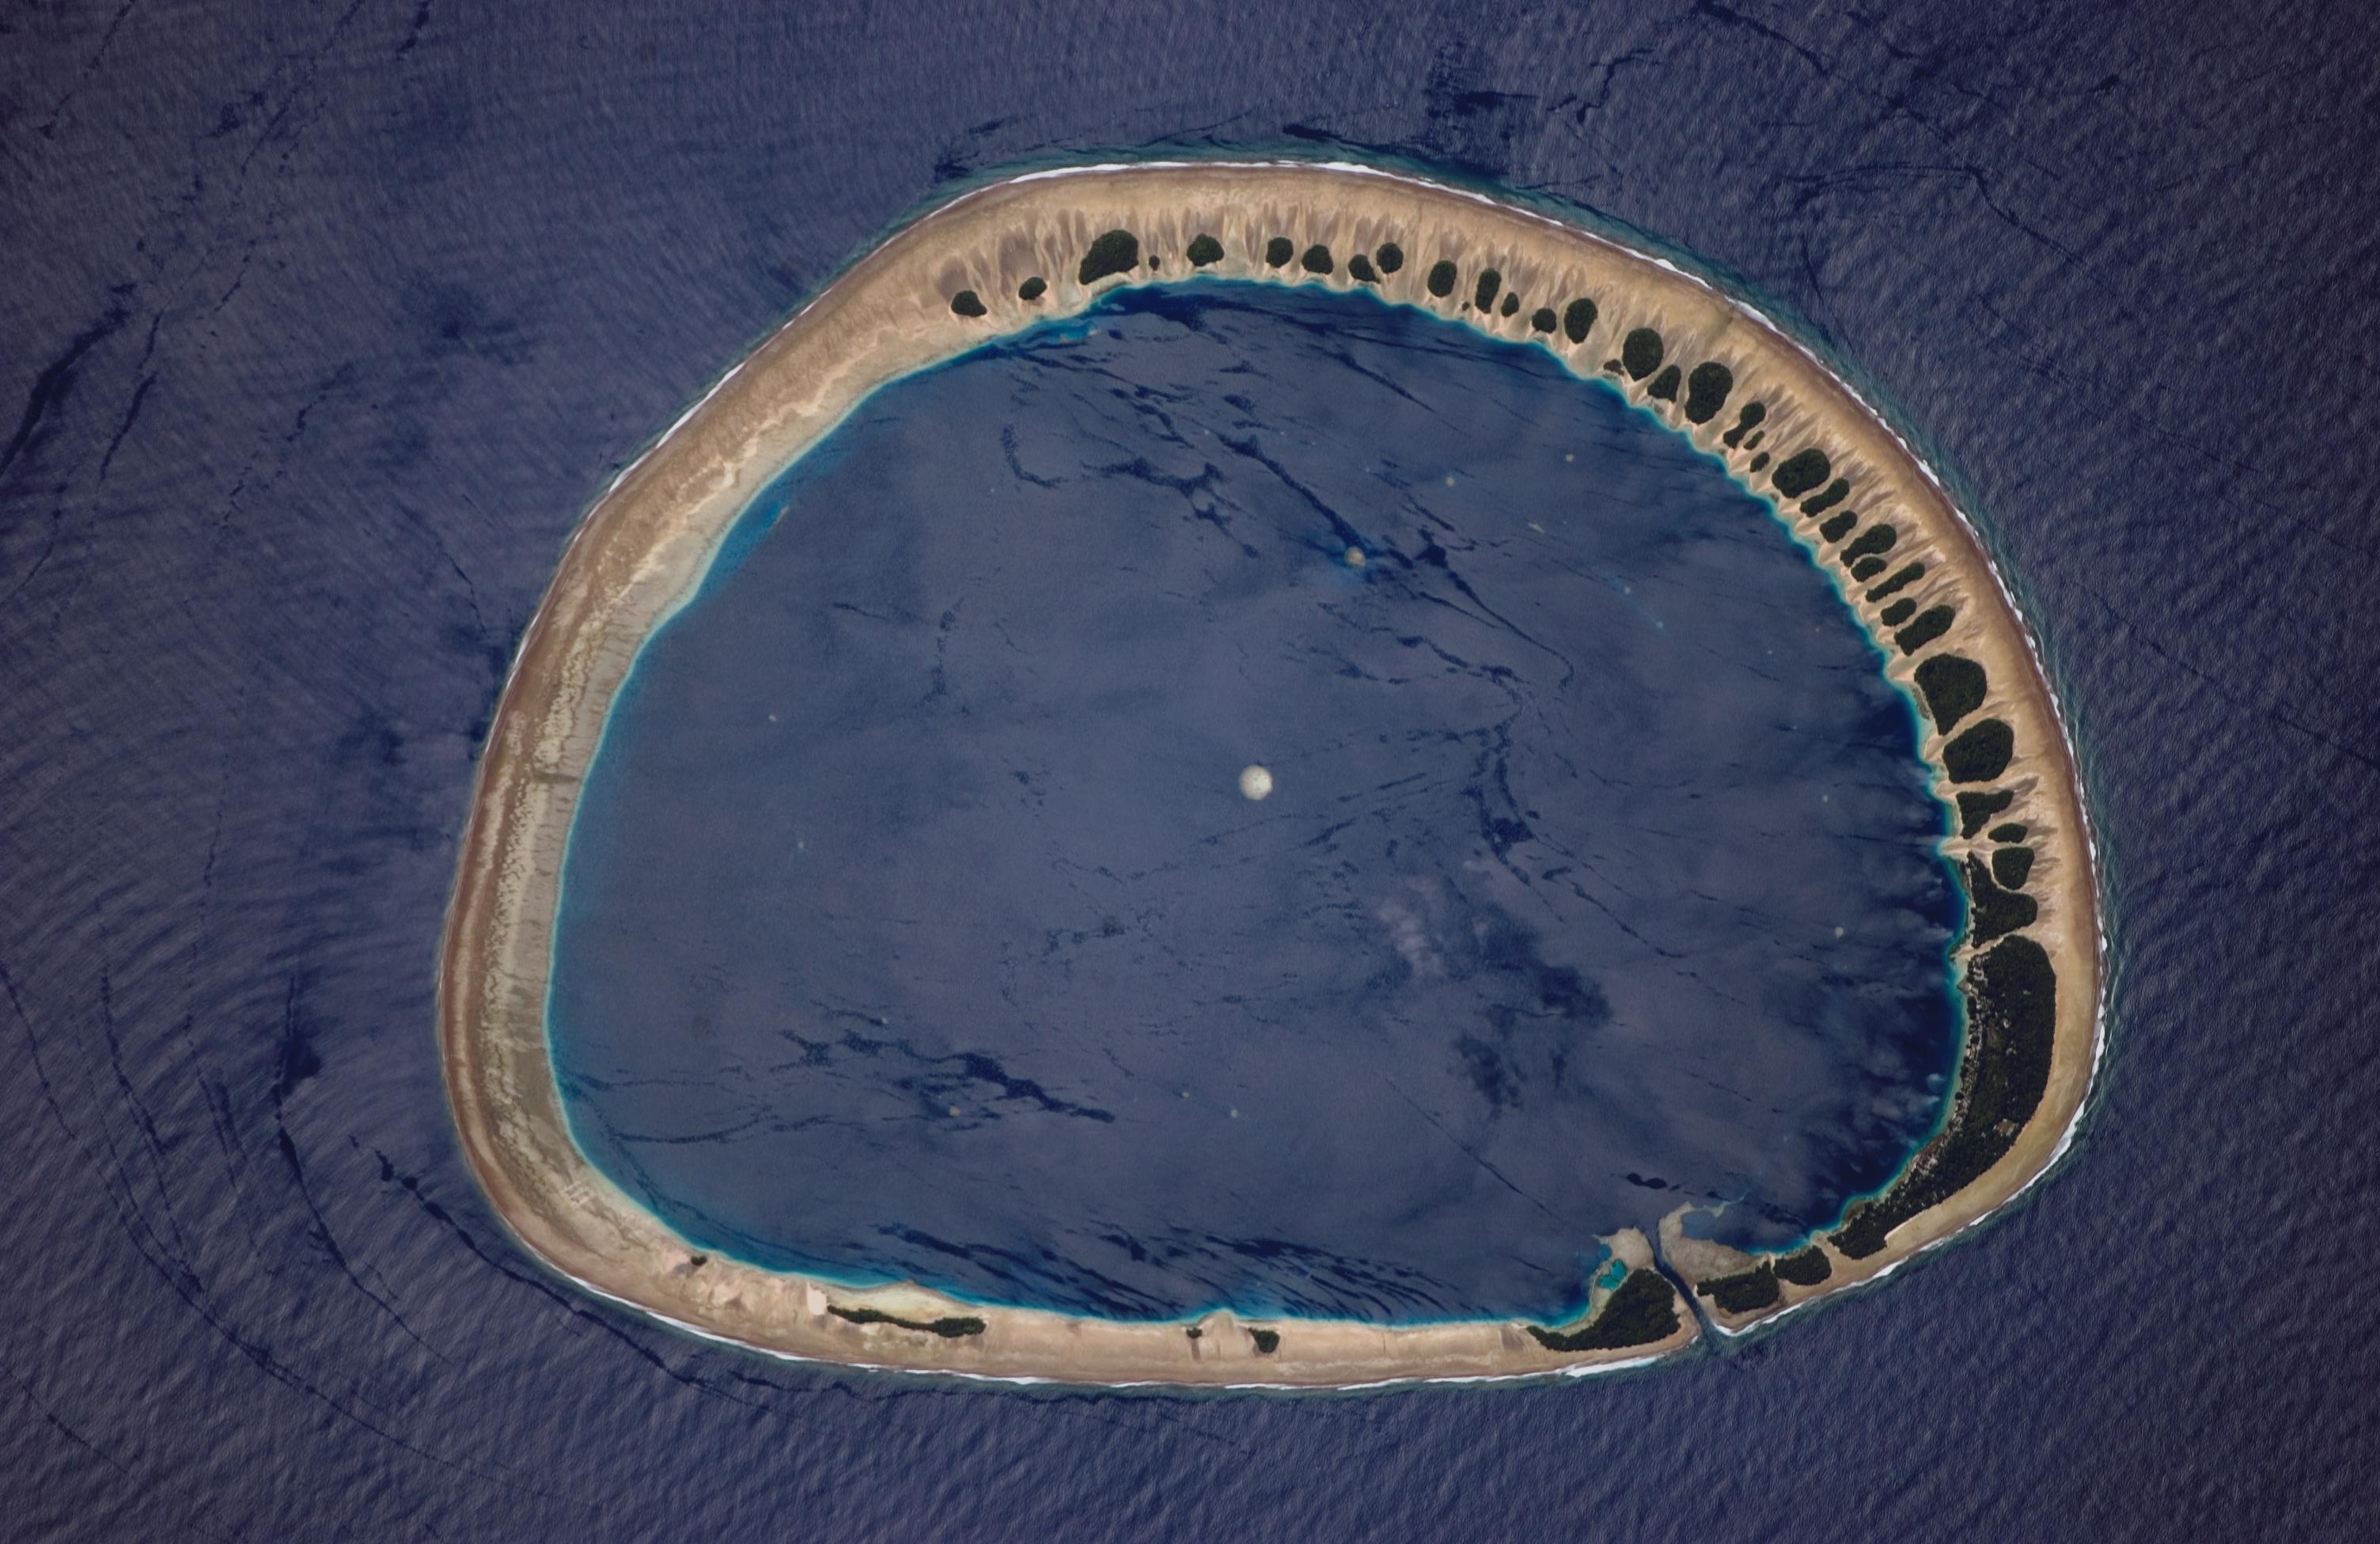
\includegraphics[width=1\linewidth]{obrazky/marine/atol}
	\caption{Atol Nukuoro, Federativní státy Mikronésie (Autor: NASA/Johnson Space Center, Image Science \& Analysis Laboratory, volné dílo)}
	\label{fig:atol}
\end{figure}

\section{Typy pobřeží}
Podle morfologie a vzniku pobřeží můžeme rozlišit celou řadu typů. 

\emph{Fjordové pobřeží} vzniklo zatopením ledovcových údolí (trogů) pobřežních pohoří. Tento typ pobřeží je typický pro Norsko a Kanadu. 

\begin{figure}[h]
	\centering
	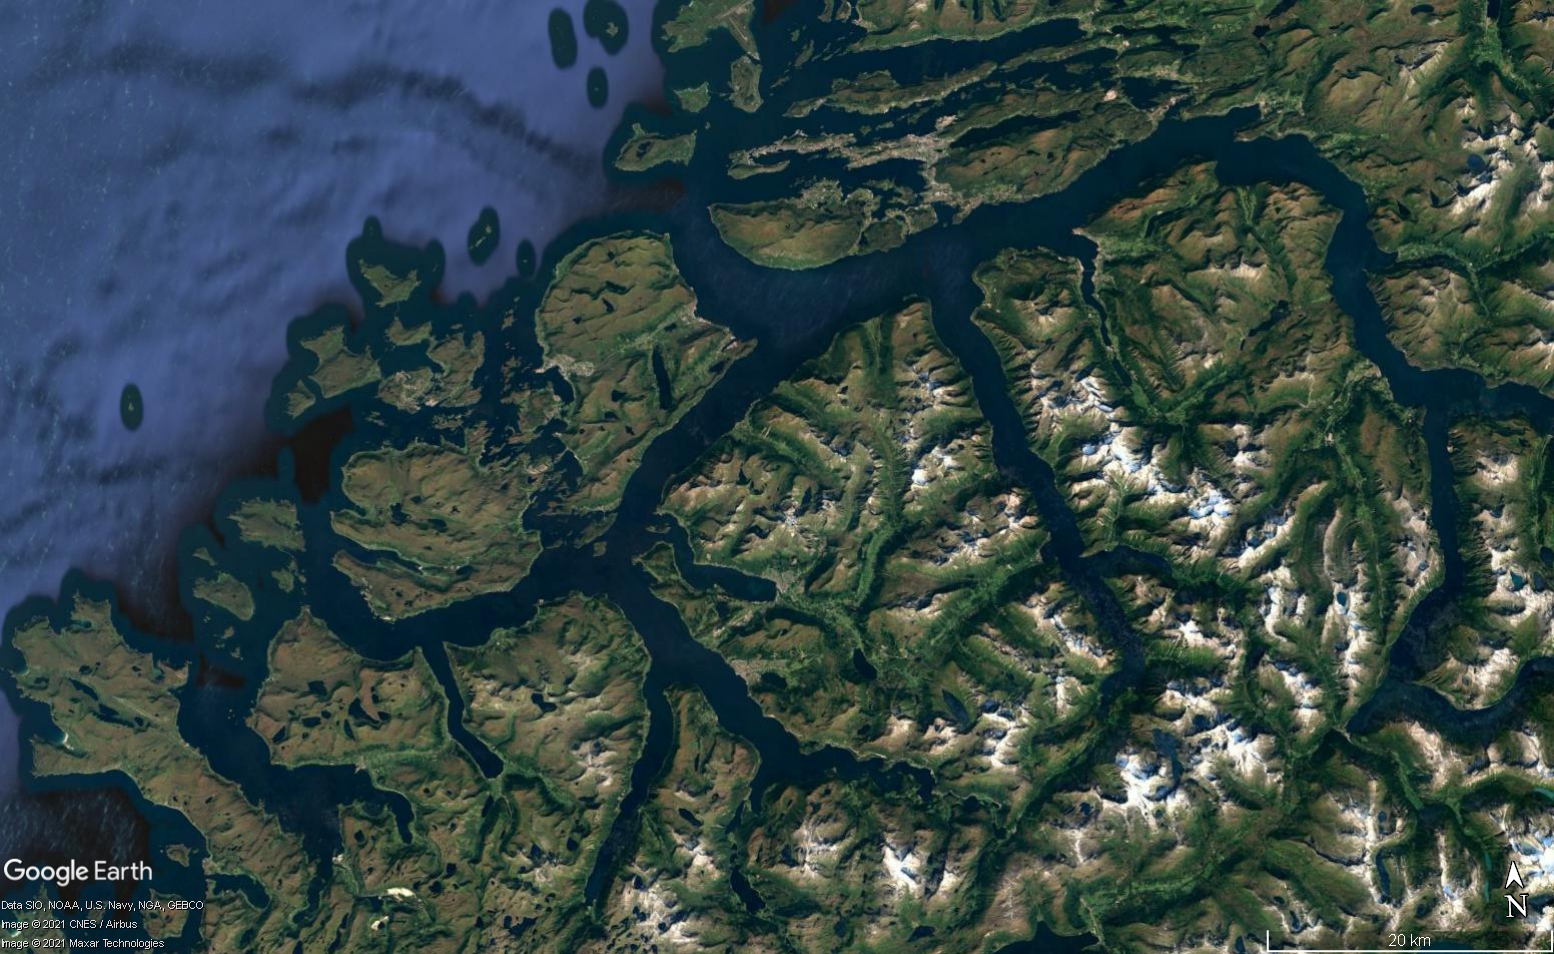
\includegraphics[width=1\linewidth]{obrazky/marine/fjord}
	\caption{Norské fjordy (Zdroj: Google Earth)}
	\label{fig:fjord}
\end{figure}


\emph{Šérové (skjarové) pobřeží}  jsou charakteristická zaoblenými skalkami, četnými malými ostrůvky. Jedná se o zaplavený erozní reliéf modelovaný kontinentálním zaledněním. Drobné ostrovy jsou zaplavené (a postglaciálním výzdvihem vyzdvižené) oblíky. Příkladem je východní pobřeží Švédska (zejména v okolí Stockholmu).

Znakem \emph{riasového pobřeží} jsou zatopená říční údolí pobřežních pohoří.

\emph{Limanové pobřeží} vzniká zaplavením pobřežních nížin. Od moře či oceánu je pobřeží zpravidla odděleno kosami.

\begin{figure}[h]
	\centering
	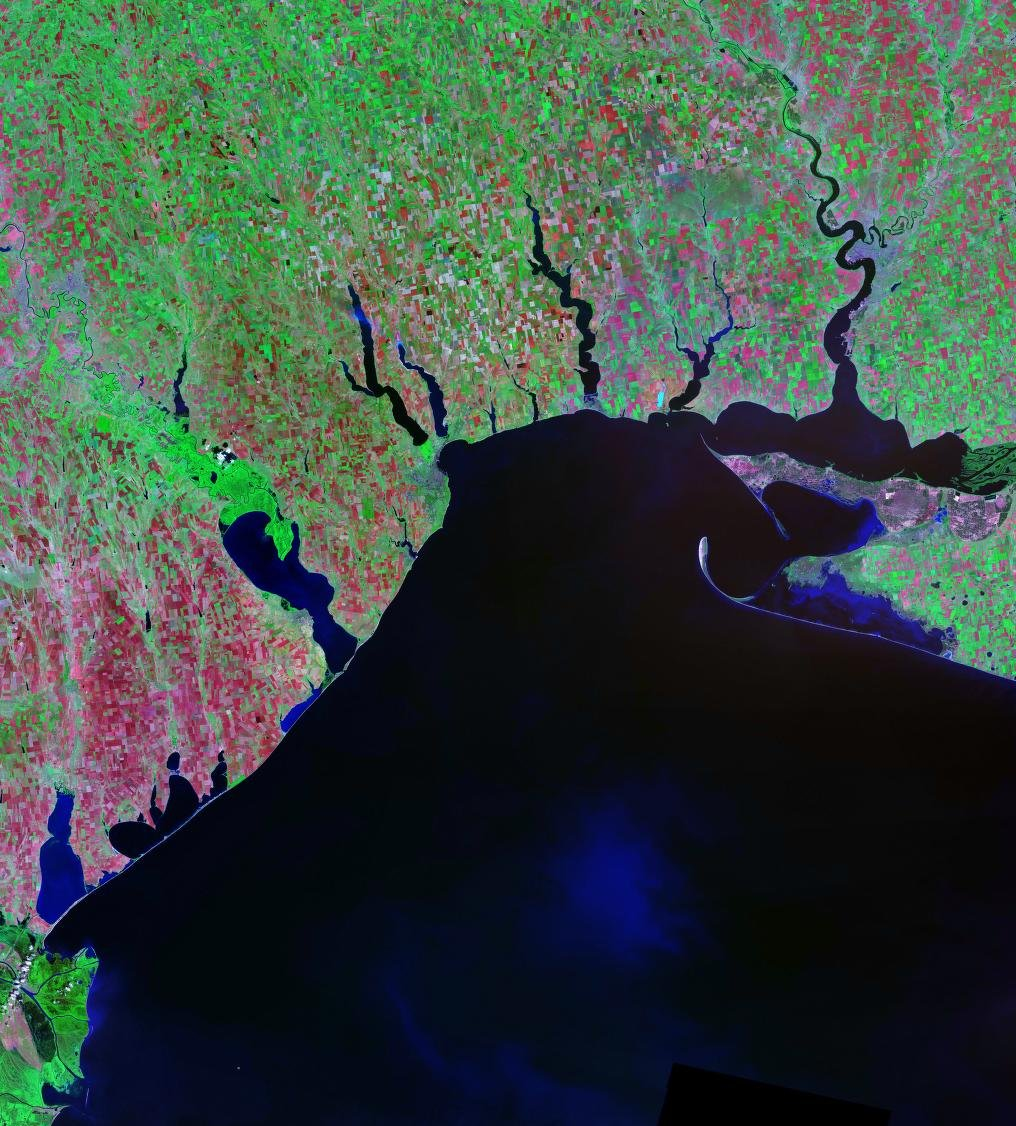
\includegraphics[width=1\linewidth]{obrazky/marine/Limans}
	\caption{Limany na severním břehu Černého moře. (Via Wikimedia Commons)}
	\label{fig:limans}
\end{figure}

\emph{Pobřeží dalmatského typu} je charakteristické četnými ostrovy, které jsou protažené ve směru pobřeží, a zálivy s úzkým ústím a větvící se na obě strany od ústí. Tento typ pobřeží vznikl zaplavením vrásových struktur probíhajících zhruba rovnoběžně s břežní čarou. 

%Pobřeží egejského typu
\emph{Pobřeží aralského typu} vzniká zaplavením deflačních sníženin eolických nížin.

\emph{Vulkanická pobřeží} jsou tvořena vulkanickými tvary, jejichž sníženiny zaplavilo moře. 

\emph{Korálová pobřeží} jsou častým typem pobřeží tropických oblastí. 

%\section{Reliéf mořského dna}
%Podmořské plošiny 
%
%\emph{Středooceánský hřbet} jsou 
%
%Hlubokomořské příkopy


\section{Změny výšky mořské hladiny}
Vznikající tvary na pobřeží reflektují průměrnou výšku hladiny moře a souše. Avšak podél pobřeží lze najít celou řadu tvarů, které dokládají to, že hladina moře byla relativně výše nebo níže vůči pevnině. Tvary na pobřeží tak mohou být \emph{ponořené} (\textit{submerged}), pokud se relativní výška moře zvýšila. Došlo tedy k tzv. \emph{transgresi} a zaplavení části pevniny. NEbo mohou být tvary \emph{vynořené} (\textit{emerged}) v případě kdy došlo k \emph{regresi}, neboli ústupu moře. 

\subsection{Příčiny změny výšky hladiny}
Možných příčin změny mořské hladiny je celá řada. \emph{Eustatické pohyby} hladiny světového oceánu jsou způsobené změnami objemu vody a projevují se v celoplanetárním měřítku. Objem vody a tím i výška hladiny se mění i s měnící se teplotou z důvodu teplotní roztažnosti vody. Nárůst průměrné teploty oceánů o \SI{1}{\degree\celsius} by způsobil zvýšení hladiny o přibližně \SI{2}{\metre}. Objem vody ovlivňuje i salinita. Zvýšení salinity způsobuje zmenšení objemu a naopak.

Podobně jak se postupem času zanáší vodní nádrž sedimenty, které unáší vodní tok, stejně se postupně zasedimentovávají i oceánské pánve. Zmenšování jejich objemu způsobuje velice pomalé zvyšování hladiny světového oceánu. Udává se, že současná globální denudace způsobuje zvýšení hladiny o přibližně \SI{3}{\milli\metre}.

Změny úrovně mořské hladiny se dějí i v důsledku tektonických pohybů. Poklesy oceánských pánví způsobují nárůst jejich kapacity, což v důsledku způsobuje pokles hladiny vůči pevnině. Naopak výzdvih či zmenčování oceánský pánví v důsledku pohubů litosférických desek vede k nárůstu hladiny.
Epeirogenetické a orogenické pohyby také ovlivňují relativní výšku hladiny moře vůči pevnině. Známé jsou bývalé antické přístavy ze středomoří, které jsou v současnosti vyzdviženy nad současnou hladinu Středozemního moře.

Hladinu světového oceánu ovlivňují i isostatické pohyby, tedy pohyby zemské kůry v důsledku jejího odlehčení či zatížení. Nejpatrnější to je na příkladu glaciisostatických pohybů. Zemská kůra byla zatlačena v důsledku zatížení kontinentálními ledovci během glaciálů. Následným zánikem kontinentálního zalednění došlo k odlehčení zemské kůry a k jejímu opětovnému výzdvihu. Tento výzdvih kompenzuje nárůst hladiny, který je způsoben  a ústupem ledovců došlo k odlehčení zemské kůry a k jejímu výzdvihu. 

Ledovcové příkrovy během glaciálů v sobě zadržovly obrovské objemy vody. Během posledního glaciálního maxima (cca 20 tisíc let zpět) byla hladina světového oceánu asi o 140 m níž než dnes. Následným táním ledovců se hladina začala zdvihat. Tato transgrese byla např. ve Skandinávii kompenzována výzdvihem pevniny v důsledku výše zmíněné glaciisostáze.

Relativní hladinu moře může ovlivnit i člověk svou činností. Například čerpání podzemní vody v pobřežních oblastech způsobuje poklesy pevniny v důsledku konsolidace sedimentů ve zvodních. Poklesem pobřeží se relativně zvyšuje hladina moře a dochází k zaplavování souše.


%\subsection{Vynořená pobřeží}
%
%\subsection{Potopená pobřeží}




\newpage
\onecolumn
\begin{boxotazky}{Kontrolní a klíčové otázky, na které bychom měli znát odpověď}
	\begin{itemize}
		\item 
		\item 
		
	\end{itemize}
\end{boxotazky}

\begin{boxslovnik}{Další klíčové pojmy k zapamatování}
	aaa & adfasd \\
	
\end{boxslovnik}
\twocolumn







